\documentclass{article}

\usepackage[utf8]{inputenc}
\usepackage{tex/mystyle} 
\usepackage{tex/mycommands}
\usepackage{fontawesome}

\author{Alexander Clark\\ \scalebox{0.7}{Columbia University - Stats 1101}} 
\title{75 Minutes of Python}

\begin{document}
\maketitle


\section{What is Python?}

Python is a general-purpose programming language. Our purposes are statistical calculations and the occasional graph. We will run code in \link{https://colab.research.google.com/}{Google Colaboratory} notebooks. This roughly mirrors running Jupyter notebooks on your own machine, but we skip the setup by running everything in the browser. If you master intro stats and become proficient in Python and SQL, there is a six-figure job waiting for you at any number of tech companies.\footnote{At least there was in early 2022. \link{https://www.reveliolabs.com/news/macro/who-gets-laid-off/}{Data scientists are over-represented in layoffs}.} 

Python is popular because the code is readable. More specifically, ``Pythonic'' code is readable. Pythonic code not only gets you from point A to B, but it uses Python as it was intended and conforms to the standards of beauty described in \emph{The Zen of Python} and \link{https://peps.python.org/pep-0008/}{elsewhere}.

\begin{footnotesize}
\begin{displayquote}
Beautiful is better than ugly.\\
Explicit is better than implicit.\\
Simple is better than complex.\\
Complex is better than complicated.\\
Flat is better than nested.\\
Sparse is better than dense.\\
Readability counts.\\
Special cases aren't special enough to break the rules.\\
Although practicality beats purity.\\
Errors should never pass silently.\\
Unless explicitly silenced.\\
In the face of ambiguity, refuse the temptation to guess.\\
There should be one---and preferably only one---obvious way to do it.\\
Although that way may not be obvious at first unless you're Dutch.\\
Now is better than never.\\
Although never is often better than *right* now.\\
If the implementation is hard to explain, it's a bad idea.\\
If the implementation is easy to explain, it may be a good idea.\\
Namespaces are one honking great idea---let's do more of those!
\end{displayquote}
\hfill The Zen of Python, by Tim Peters
\end{footnotesize}

Python can seem endlessly complex. \link{https://www.oreilly.com/library/view/fluent-python-2nd/9781492056348/}{\emph{Fluent Python}} is 1,012 pages. Luckily, we don't need to aspire to fluency. Let's learn just enough of the language to order off the kids' menu. 


\section{Python as a Calculator}

\subsection{Variables}

A Python variable holds a value. It can be a string, a number, or perhaps a more complicated data type. Variable assignment is done with the equals sign, \lstinline[language = Python]{=}. Below, we create a string variable called \code{greeting} and a integer variable called \code{my_favorite_number}. 

\smallskip

\pyfile{vars.py}

\smallskip
\noindent Now compare the output you get from the following.
\pyfile{print-vars.py}


\noindent Note that while $x = x+1$ is nonsense as a mathematical equation, in Python \code{x = x+1} simply adds one to the value of \code{x}. What's the value of \code{x} at the end of the following program?\footnote{\rotatebox{180}{Three.}}

\pyfile{reassignment.py}

\subsection{Comments}
Commenting your code is helpful if you care about your colleagues or your future self. Comments should add clarity to the intention and workings of code. A comment is a piece of code that isn't actually executed---it's a comment left for the reader or the person who inherits and modifies your code.
Everything after a \lstinline[language = Python]{#} will be ignored by Python.

\pyfile{comment.py}

\smallskip
 \noindent You might also use end-line comments like the following

\pyfile{inline.py}


\smallskip

\noindent Perfect comment technique does not correct for bad code though. Compare the following blocks of code. 

\pyfile{compensation.py}

\pyfile{good-names.py}

The first block is commented and the second is not. Still, the second code block is better because the variable names are chosen so you don't \emph{need} comments. Good naming becomes even more important as the program becomes longer and variables are used over and over. 



\subsection{Calculations}
Below is a list of some typical operations. What might stand out is that exponentiation is done with \code{**} and not \code{^}. It happens that \code{^} still works, but it does something else. 


\begin{center}
{\setlength{\tabcolsep}{2em}
\begin{tabular}{lll}
\toprule
Operator & Description \\
\midrule
\code{+} &    Addition \\
\code{-} & Subtraction \\
\code{*}  &    Multiplication \\
\code{/}  &   Floating point (normal) division \\
\code{**} & Exponentiation \\
\bottomrule
\end{tabular}}
\end{center}

We can use parenthesis for readability and to order operations in the usual way.

\pyfile{parens.py}

For our first substantive program, let's calculate the test statistic for $\hat{p} = 0.34$ with $n=116$ if we assume a null hypothesis of $p = \frac{1}{3}$. We will obtain \code{z = 0.15231546211727914}.

\pyfile{z-stat.py}

\subsection{Truth and Decision Structures}

You'll notice the test statistic we just calculated is small. For a 95\% confidence level and a two-sided test, we would fail to reject the null hypothesis because $\vert z \vert < 1.96$. It would be nice if Python could make that call without us even having to look at the statistic. We can do that with if statements. If statements are based on truth statements, or boolean expressions.

\pyfile{if-true.py}

\pyfile{if-false.py}

We don't work directly with \code{True} and \code{False} in practice. We have to make use of comparison operators. 

\begin{center}
{\setlength{\tabcolsep}{2em}
\begin{tabular}{lll}
\toprule
Operator & Description \\
\midrule
\code{==} &    Equality, \code{1 == 1} \\
\code{>} & Greater Than, \code{1 > 0} \\
\code{<}  &  Less Than, \code{1 < 2} \\
\code{>=}  &   Greater Than or Equal, \code{1 >= 1} \\
\code{<=} & Less Than or Equal, \code{9 - 1 <= 7 + 1} \\
\bottomrule
\end{tabular}}
\end{center}

\noindent Observe.

\pyfile{if-calc.py}

\noindent Using the \code{abs()} function above to take an absolute value, Python knows $1 = \vert -1 \vert$ and executes only the first print statement. Finally, let's have Python make the call on our hypothesis test. 

\pyfile{reject-rule.py}

\section{Libraries for Statistical Functions and Graphs}
We've hit a ceiling in Python's usefulness. You, the coder, supplied the critical value 1.96 in the previous program and we couldn't calculate a P-value. To go further, we have to import additional libraries that contain the stuff we want to use. SciPy, and specifically the stats module, will replace a $z$-table and then some. Below, we import the SciPy stats module and use it to calculate $P(Z < 1.96)$, using the standard normal CDF.

\pyfile{scipy-norm.py}

\noindent We can go in the opposite direction with \code{stats.norm.ppf}. 

\pyfile{crit-val.py}

Occasionally, it's useful to simulate data. SciPy again suits this purpose. For this call, we make use of keyword parameter \code{size}, specifying that we want 75 iid draws from the standard normal distribution. 

\pyfile{rand-draws.py}

\noindent If you display \code{random_draws}, you'll see we have an array---a new data type.

\begin{center}
\begin{tabular}{c}
\begin{lstlisting}[backgroundcolor=\color{white}, numbers = none]
    array([ 0.26670047,  0.90571598,  0.58999261, -0.11483403, -0.11317713,
        0.24380578, -1.34662353, -2.38132282, -1.06133942, -0.51280499,
       -0.20017384, -0.99053684,  1.39045452, -0.03411639,  0.86640634,
       -0.58858272, -0.07981447, -1.15327852,  0.75582911,  0.6196648 ,
       -1.21089585,  0.71239498,  0.53601251, -0.60518285,  0.81547665,
        0.87444887,  0.17482955, -0.30222337,  0.70213597, -0.48985895,
        0.58287787,  0.43369743,  0.47753534,  0.4218932 ,  1.28159422,
        0.98054053,  0.47001209,  0.63269663,  1.48985604, -2.17641724,
        0.70551392,  0.65769517, -0.19576411,  0.09185508, -0.53660252,
       -0.15239094,  1.01012891,  0.52824524,  1.28593209, -1.12874119,
        1.4837867 ,  1.11762774, -1.44385417, -0.54467961,  2.1815505 ,
        0.82446247,  1.52427836, -0.89112124,  0.79242734,  0.81785614,
       -0.11150023, -0.24244312,  0.66204106,  1.46663459,  1.30903711,
        1.49169821, -0.36590489, -0.16852676,  2.11081052, -0.45121903,
        0.88317932, -0.55096038,  0.6298471 , -0.1914023 , -0.71709689])
\end{lstlisting}
\end{tabular}
\end{center}


\noindent We'll sneak in a histogram. The standard data visualization library for Python is matplotlib. We use the pyplot module for a bare-bones histogram in Figure \ref{fig:hist}.

\pyfile{mpl-hist.py}


\begin{figure}
    \centering
    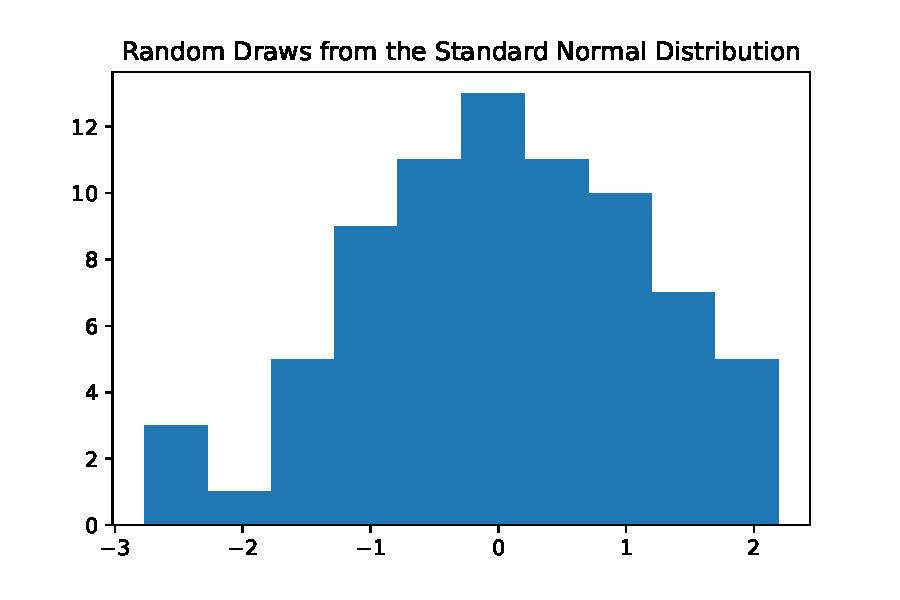
\includegraphics[width = .59\textwidth]{figures/first_histogram.pdf}
    \caption{Our first histogram.}
    \label{fig:hist}
\end{figure}

We can simulate Bernoulli draws and run a hypothesis test. Python has a small selection of mathematical functions available apart from any library. Previously, we used \code{abs()}. Below, we use \code{sum()} and then \code{len()} which counts the number of elements in  an array.

\pyfile{bernoulli.py}

\noindent We can run many with the help of a special repetition structure called a \emph{for loop}. The code below simulates 30 flips of a fair coin 10,000 times. \code{k} records how often our test statistic, under a null of $p= 0.5$, would lead us to incorrectly reject the null hypothesis using $\alpha = 0.05$ and a two-sided alternative. What value do you expect for \code{k/N}?\footnote{\rotatebox{180}{\code{k/N} should be close to 0.05, using a Normal approximation. Large simulations will show this approximation to be inexact.}}

\pyfile{simulation.py}



\section{Libraries for Data}

The main library for data wrangling and anything tabular (like a spreadsheet) is pandas. Pandas is famous---it's no wonder the bear is named after this library. Primarily, we will read csv and xlsx files into \emph{DataFrames}. DataFrames can also be constructed by hand like in the program below.

\pyfile{pandas-df.py}

Individual columns can be accessed as a \emph{Series} with \code{df['frosty_expenditure']} or \code{df.frosty_expenditure}.\footnote{This pattern will not work if there is a space in the column name or if the column doesn't adhere to other naming requirements.} We can then create new columns based on existing columns. 

\pyfile{new-column.py}

\noindent DataFrames and Series also have special \emph{methods} available. 

\pyfile{pd-methods.py}

\section{Further Resources and Caution}

\subsection{Resources}

I got my start with \link{https://www.datacamp.com/}{DataCamp} courses. DataCamp uses a subscription model that is affordable. There are also many excellent, free resources available that will help you learn Python. \link{https://wesmckinney.com/book/}{\emph{Python for Data Analysis}} by Wes McKinney was updated in 2022, making it one of the most current resources. I also recommend Jake VanderPlas's \link{https://jakevdp.github.io/WhirlwindTourOfPython/}{\emph{Whirlwind Tour of Python}} and \link{https://jakevdp.github.io/PythonDataScienceHandbook/}{\emph{Python Data Science Handbook}}. For plotting with matplotlib, try \link{https://github.com/alexanderthclark/Matplotlib-for-Storytellers}{my book}. 

\subsection{Caution}

Recall when we calculated sample variance as $\sum_{i=1}^n \frac{(x_i - \bar{x})^2}{n-1}$. We used $n-1$ instead of $n$ in the denominator as correction for unbiasedness. Not all Python libraries do this by default! NumPy is one such library that does not use the correction by default. The lesson here is that, for this class, do your research if you are using other libraries and functions. There are many ways to do what sounds like the same thing in statistics and some disjointedness across all of the Python libraries. 

Below is another example where default behavior in the StatsModels library does not match our intro conventions. For now, our calculations are simple enough that I don't recommend finding random libraries and functions to shorten your code. 

\pyfile{prop-ztest.py}

\end{document}
